% upLaTeX文書
% \documentclass[uplatex,a4paper]{jsarticle}
\documentclass[pdflatex,ja=standard]{bxjsarticle}
% デフォルトのフォント設定のまま!
\usepackage{color}
\usepackage{url}
\usepackage{graphicx}
\usepackage{algorithm}
\usepackage{algorithmic}

\definecolor{myred}{rgb}{0.85,0,0.1}
\definecolor{mypink}{rgb}{1,0.92,0.92}
\setlength{\fboxsep}{2pt}


\title{情報探索と検索 学期末レポート課題}
\author{201821636 村松直哉}
\date{\today}
\begin{document}
\maketitle
%
%


% Google++という名前の新しいサーチエンジンを提案・設計しなさい。
% - 設計の動機
% - ベースとなるユーザモデル
% - 機能(何をどのように支援・高度化するのか)
% - 仕組み(アルゴリズムなど)
% - 評価計画
% を詳細に記述しなさい。
% レポートで述べられたアイディアは,授業中やリーディングリストに挙げた資料で説明されているモデル,理論,技術,研究成果を具体的に参照して,その根拠とすること。またレポート課題に用いた引用文献一覧を含めること。必要であれば,1-2個の図表を用いてもよい。

\section{はじめに}
Googleの検索エンジンには,{\rm Knowledge Panel}(KP)~\cite{Amit2012}という機能がある.
これは様々な情報源から収集したセマンティック検索情報を用いて,検索結果を拡張する.
図\ref{fig:knowledgepanel}に,KPの表示例を示す.

これは十分に情報が整理され,わかりやすいものである.
\cite{Lagun}より,スマートフォン画面での配置を工夫されたKPの表示は,ユーザの注意を十分に引いていることがわかる.
しかし,PC画面に表示された場合(図\ref{fig:knowledgepanel})右端に表示される.
従来の表示手法になれたユーザは,検索結果を上から見ていくと考えられる~\cite{Granka2004}.
そのため,KPに十分に注意を引くことができない.

私は,KP情報を音声情報に変換し自動的に再生する{\rm Google++}を提案する.
対象クエリに関する基礎的な情報を含んだKPを,最初にユーザに提示する.
これにより,ユーザは検索対象情報を得るまでのクリック数を減らすことを目的とする.

\begin{figure}[htb]
\begin{center}
    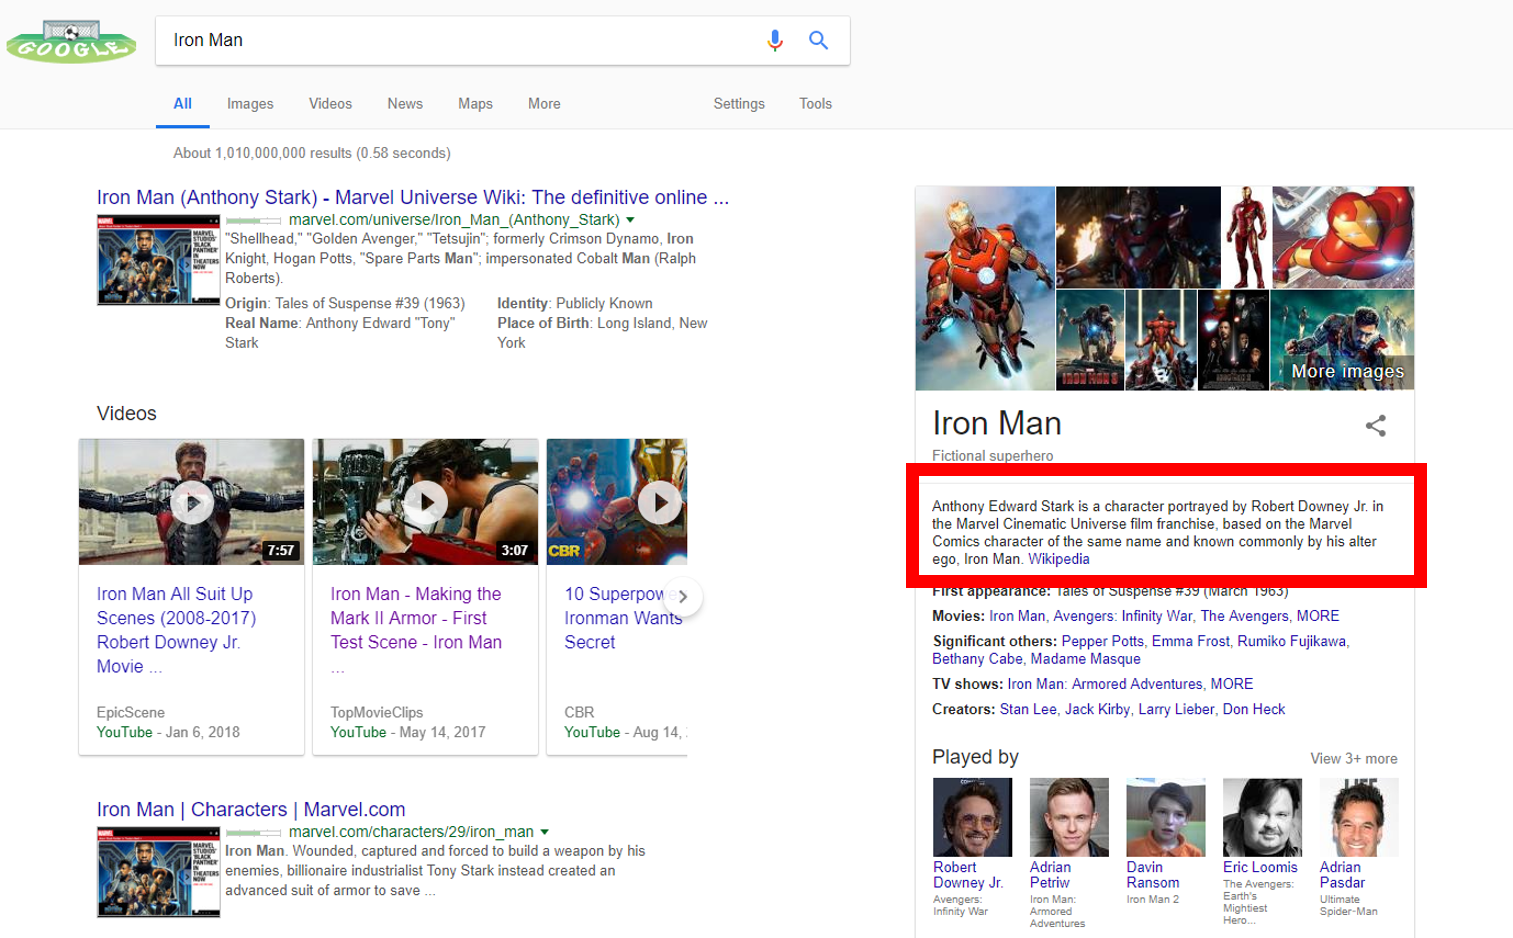
\includegraphics[width=14cm]{figs/ironman.png}
\end{center}
\caption{PC画面でのGoogle Knowledge Panelの表示例}
\label{fig:knowledgepanel}
\end{figure}


\section{システム構成}

図\ref{fig:system}にユーザを含めた処理フローを示す.
ユーザは従来の検索エンジン同様に,作業関連する情報ニーズを表した検索質問(クエリ)をシステムに入力する.
クエリはまずGoogleの検索エンジンによって検索結果を得る.
ここでKPが表示される場合,本システムはこれを解析し,text-to-speech(TTS)アルゴリズムにより音声情報を,検索結果とともにユーザに渡す.

これにより,ユーザが検索対象情報を得るまでのクリック数を減らすことを目的とする.
言語対応については,英語を対象にしたシステムを想定とする.

音声読み上げについては,TTSによりテキスト情報から変換を行い,生成された音声を再生する.
使用するアルゴリズムは,自然性の高い読み上げが可能なWaveNet~\cite{Oord2016}を用いる.

生成された音声は,十分に短い時間内で読み上げられる必要がある.
KP内の文章が長すぎる場合には,さらに情報を要約する.
この手法については,\ref{sec:summarize}で詳しく述べる.

\begin{figure}[htb]
\begin{center}
    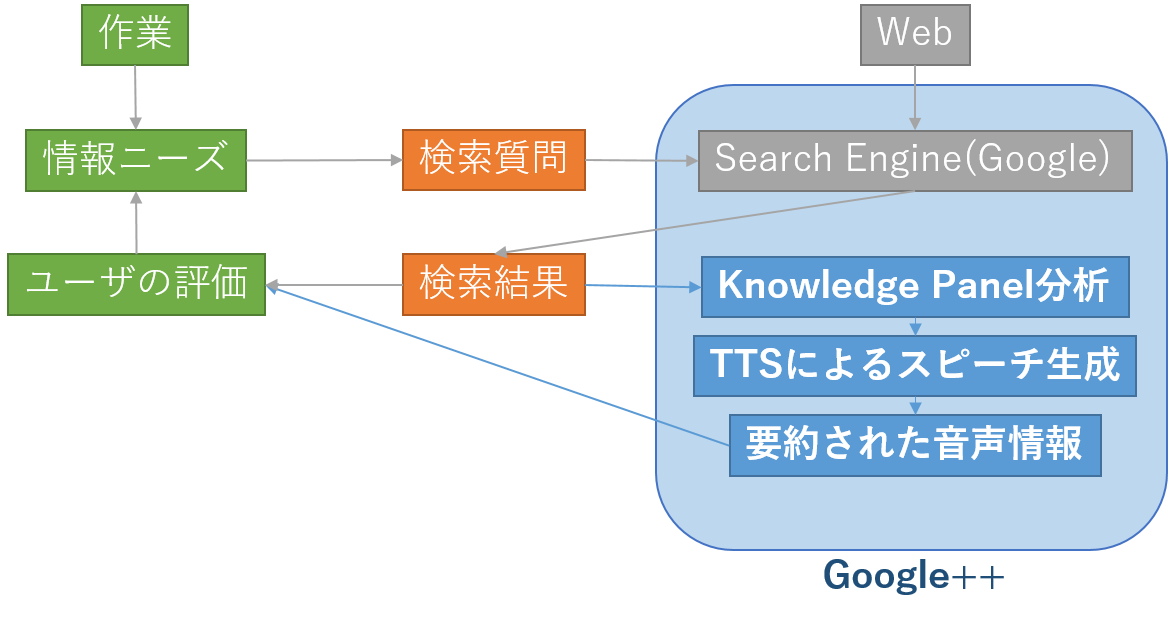
\includegraphics[width=14cm]{figs/system.png}
\end{center}
\caption{処理フロー}
\label{fig:system}
\end{figure}

\subsection{Knowledge Panel抽出手法}

KPの有無やテキスト抜き出しには,通常のスクレイピング手法を用いる.

KPが検索結果に表示される際には,表示ページのHTMLに,クラス名{\rm kp-blk}を含むdivタグが出現する.
これにより,KPの存在を確認できる.
また,KPに記述される短い説明文も同様に,クラス名{\rm kno-rdesc}を基に抽出できる.

\subsection{文章要約手法} \label{sec:summarize}

読み上げ速度は,生成された音声データにより依存する.
これを計測したところ,約$2.3\,\mathrm{words/s}$であった.
情報をユーザに提示する際に,検索結果を確認する時間は,約8秒である~\cite{Granka2004}.
つまり,8秒以内に読み上げる事のできる単語数は,約$18\,\mathrm{words}$である.

英語の1文あたりの単語数は$15--20\,\mathrm{words}$である~\cite{Mesa}.
そのため,本システムで読み上げられる単語数は,基本的に$20\,\mathrm{words}$以下とする.

KPには,対象情報に関する短い説明文である,{\rm knowledge description}(KD)が付く(図\ref{fig:knowledgepanel}における赤枠の部分).
本システムでは,KDの文章を利用して,音声情報を生成する.

アルゴリズム\ref{alg:summarize}は,KDの文章が長すぎる場合の要約手法を示している.
基本的には,最初の文を利用する.
それが長い文の場合,カンマを基準に文を分割する.
分割した各テキストから,対象クエリを最も多く含むテキストを利用する.
それでも長いテキストになる場合には,音声の読み上げスピード上げることで,8秒以内に情報提示を終えるようにする.

\begin{algorithm}
\caption{文章要約アルゴリズム}
\label{alg:summarize}
\begin{algorithmic}
    \STATE $D \leftarrow$ the knowledge description
    \STATE $d \leftarrow D$の最初の文
    \STATE $q \leftarrow $stemming処理したクエリ
    \STATE $speachspeed \leftarrow 1.0$
    \STATE $th \leftarrow 20$
    \IF{$d$の単語数 $\leq th$}
        \RETURN $d$
    \ELSE
        \STATE $c \leftarrow$ $d$をカンマで分割した最初の要素
        \STATE $d \leftarrow$ $c$で$q$を最も多く含む要素
        \IF{$d$の単語数 $> th$}
            \STATE $speachspeed \leftarrow d / th$
        \RETURN $d$
        \ENDIF
    \ENDIF
\end{algorithmic}
\end{algorithm}


\section{検証実験}

本システムの有効性を検証するために,様々な被験者実験を設計し,実施する.
被験者実験は,KPを基にした短い音声情報提示により,ユーザの情報探索方法や要する時間に,どのように影響するかを調べる.
音声情報は,KPを基にしているため有名な人物や場所などの,ある実在するもの([louvre]や[angelina jolie]など)に関連するクエリ情報を提供する.
音声情報により素早く情報を概要をつかめるため,実験でのタスクでは,一般的に知られていないクエリを対象とした.

検証実験には,以下のプロトコルで行った.
参加者には,20の検索タスクのリストが載ったウェブページを提示する.
リスト内の各エントリは,タスクの説明,2つのハイパーリンク--1つは検索結果ページ(タスクに関連する事前定義されたクエリを指す),2つ目はタスク後のアンケートページである.
参加者は,タスクの説明を読んで,検索エンジンを利用してタスクの答えを見つけて,タスク後のアンケートをしてもらった.

各タスクの難易度が同じであることを確認するために,著者は各タスクについて,対応する1つ検索結果ページに答えが含まれていることを確認する.
したがって,参加者に行ってもらうタスクは非常に簡単で(1分未満で済む),参加者は1タスクにつき3分を超えないように指示する.
答えを見つけたら,参加者はブラウザの「戻る」ボタンを使って実験トップページに戻り,2番目のハイパーリンクをたどってアンケートを完了してもらう.
アンケートのページでは,参加者に7ポイントのリッカート尺度で検索結果全体の満足度を評価するよう依頼する(1は不満であり,7件は満足である ).
クエリはタスクごとにあらかじめ定義されており,クエリの再定義は許可しない.

実験の初期段階では,2つの要素(ユーザーの情報ニーズに対する音声情報の妥当性,および音声情報の存在)を含む$2\times 2$課題設計を使用する.
両方の要素には2つのレベルがあります。関連性 - 関連性または無関係性、存在 - 存在または不在。各参加者は20の検索タスクを実行した(条件ごとに5つのタスク)。タスク提示の順序は、任意の学習またはタスクオーダーの影響を排除するためにランダム化された。
参加者は、使用するPCと実験フローに慣れるために,本実験を開始する前に4つの練習課題を行ってもらう.
最初の研究で20のタスクを完了した後、参加者には、知識グラフの結果ではなくインスタントアンサーの結果に焦点を当てた点を除き、研究の第2部に進む前に5分間休憩を与えた。 2番目の部分では、IAは常に存在しており、単一要因のみを変更しました。IA適合性。これにより、1条件あたりの作業の数を2倍に増やすことができました(KGで5人からIAで10人)。

\subsection{被験者}
インフォームド・コンセントを得た$18--65$歳の様々な職種の30人(男性15人,女性15人)を対象として,被験者を募集する.
被験者らは,それぞれいくつかの検索エンジン使用経験があり,利用サービスを回答してもらう.
被験者らは,正常または矯正視力(メガネやコンタクトレンズ)を有し,PC画面を操作できることを確認する.

\subsection{装置}

\begin{table}[htb]
\begin{center}
\caption{被験者実験で使用する質問タスクの例}
\begin{tabular}{l|l}
    \hline
    Query && Task Description \\
    \hline
    Suspension bridge && In what state is the bridge? \\
    Tony Stark && Who made him? \\
    university of cambridge && WWhat was the enrollment of the University of Cambridge in 2012? \\
    \hline
\end{tabular}
\end{center}
\end{table}

\section{結論}


\clearpage

\bibliographystyle{ieee}
\bibliography{references}

\end{document}